\documentclass[letterpaper, 12pt]{article}
\usepackage{amsmath}
\usepackage[x11names]{xcolor}
\usepackage{pgfplots}

\pgfplotsset{compat=1.13}

\renewcommand*{\arcsin}{\sin^{-1}}
\renewcommand*{\arccos}{\cos^{-1}}
\renewcommand*{\arctan}{\tan^{-1}}
\newcommand*{\arccot}{\cot^{-1}}
\newcommand*{\arcsec}{\sec^{-1}}
\newcommand*{\arccsc}{\csc^{-1}}
\newcommand*{\diff}{\mathrm{d}}
\newcommand*{\Diff}[1]{\mathrm{d^#1}}
\newcommand*{\e}{\mathrm{e}}

\title{Polar Coordinates}
\author{Alvin Lin}
\date{Calculus II: August 2016 - December 2016}

\begin{document}

\maketitle

\section*{Polar Coordinates}
Instead of an x,y coordinate, polar coordinates are defined by an angle and a
radius.

\begin{center}
  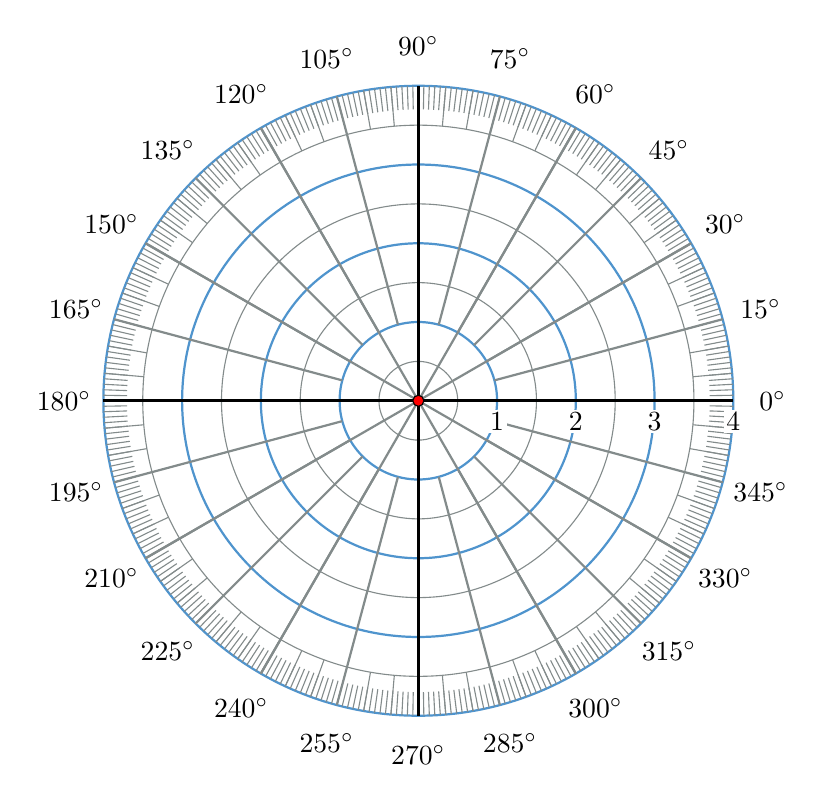
\begin{tikzpicture}
    \foreach \r in {1, 2,...,4}
      \draw[SteelBlue3, thick] (0,0) circle (\r);
    \foreach \r in {0.5, 1.5,...,4}
      \draw[Azure4, thin] (0,0) circle (\r);
    \foreach \a in {0, 1,...,359}
      \draw[Azure4] (\a:3.7) -- (\a:4);
    \foreach \a in {0, 5,...,359}
      \draw[Azure4] (\a:3.5) -- (\a:4);
    \foreach \a in {0, 15,...,359}
      \draw[thick,Azure4] (\a:1) -- (\a:4);
    \foreach \a in {0, 30,...,359}
      \draw[thick,Azure4] (0, 0) -- (\a:4);
    \foreach \r in {1, 2,...,4}
      \draw (\r,0) node[inner sep=1pt,below=3pt,rectangle,fill=white] {$\r$};
    \foreach \a in {0, 90,...,359}
      \draw[very thick] (0, 0) -- (\a:4);
    \foreach \a in {0, 15,...,359}
      \draw (\a: 4.5) node {\( \a^\circ \)};
    \draw[fill=red] (0,0) circle(0.7mm);
  \end{tikzpicture}
\end{center}

\[ x = r\cos(\theta) \quad y = r\sin(\theta) \]
\begin{center}
  \begin{tikzpicture}
    \draw[thick,->,>=latex] (-3,0)--(3,0) node[above] {\( x \)};
    \draw[thick,->,>=latex] (0,-3)--(0,3) node[left] {\( y \)};
    \fill (1,1) circle[radius=2pt] node[anchor=south]{\((r, \theta)\)};
    \fill (-1,-1) circle[radius=2pt] node[anchor=east]{
      \( (-r, \theta)\) or \((r, \theta + \pi) \)
    };
  \end{tikzpicture}
\end{center}

\subsection*{Problem 1a}
Give two other representations of \( (2, \frac{\pi}{3}) \).
\begin{center}
  \begin{tikzpicture}
    \draw[thick,->,>=latex] (-2,0)--(2,0) node[above] {\( x \)};
    \draw[thick,->,>=latex] (0,-2)--(0,2) node[left] {\( y \)};
    \fill (1,1.414) circle[radius=2pt] node[anchor=south]{
      \( (2, \frac{\pi}{3}) \)
    };
  \end{tikzpicture}
\end{center}
\[ (2, \frac{\pi}{3}) = (-2, \frac{4\pi}{3}) = (2, \frac{7\pi}{3}) \]

\subsection*{Problem 1b}
Give two other representations of \( (-1, \frac{\pi}{2}) \).
\begin{center}
  \begin{tikzpicture}
    \draw[thick,->,>=latex] (-2,0)--(2,0) node[above] {\( x \)};
    \draw[thick,->,>=latex] (0,-2)--(0,2) node[left] {\( y \)};
    \fill (0,-1) circle[radius=2pt] node[anchor=east]{
      \( (-1, \frac{\pi}{2}) \)
    };
  \end{tikzpicture}
\end{center}
\[ (-1, \frac{\pi}{2}) = (-1, \frac{5\pi}{2}) = (1, \frac{3\pi}{2}) \]

\subsection*{Problem 7}
Shade the region \( 1 \leq r \leq 2 \).
\begin{center}
  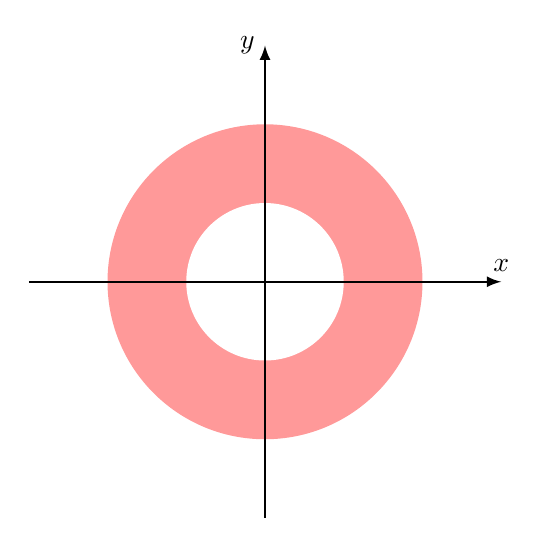
\begin{tikzpicture}
    \fill[red!40] (0,0) circle[radius=2];
    \fill[white] (0,0) circle[radius=1];
    \draw[thick,->,>=latex] (-3,0)--(3,0) node[above] {\( x \)};
    \draw[thick,->,>=latex] (0,-3)--(0,3) node[left] {\( y \)};
  \end{tikzpicture}
\end{center}

\subsection*{Problem 8}
Shade the region \( r \geq 0; \frac{\pi}{3} \leq 0 \leq \frac{2\pi}{3} \).
\begin{center}
  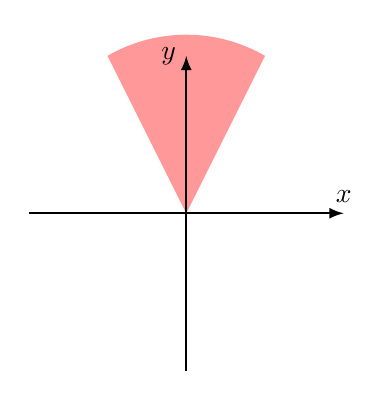
\begin{tikzpicture}
    \fill[red!40] (0,0) -- (1,2) arc (60:120:2) -- cycle;
    \draw[thick,->,>=latex] (-2,0)--(2,0) node[above] {\( x \)};
    \draw[thick,->,>=latex] (0,-2)--(0,2) node[left] {\( y \)};
  \end{tikzpicture}
\end{center}

\subsection*{Problem 14}
Find the distance between the two points:
\begin{center}
  \begin{tikzpicture}
    \draw[thick,->,>=latex] (-3,0)--(3,0) node[above] {\( x \)};
    \draw[thick,->,>=latex] (0,-3)--(0,3) node[left] {\( y \)};
    \fill (2,0.5) circle[radius=2pt] node[anchor=east]{
      \( (r_{1}, \theta_{1}) \)
    };
    \fill (0.2,2) circle[radius=2pt] node[anchor=west]{
      \( (r_{2}, \theta_{2}) \)
    };
  \end{tikzpicture}
\end{center}
\[ P_{1}(x_{1}, y_{1}) \quad P_{2}(x_{2}, y_{2}) \]
\[ x_{1} = r_{1}\cos(\theta_{1}) \quad x_{2} = r_{2}\sin(\theta_{2}) \]
\[ y_{1} = r_{1}\sin(\theta_{1}) \quad y_{2} = r_{2}\sin(\theta_{2}) \]
\begin{align*}
  P_{1}P_{2} &= \sqrt{(x_{2}-x_{1})^{2}+(y_{2}-y_{1})^{2}} \\
  &= \sqrt{(r_{2}\cos(\theta_{2})-r_{1}\cos(\theta_{1}))^{2}+
    (r_{2}\sin(\theta_{2})-r_{1}\sin(\theta_{1}))^{2}} \\
  &= \sqrt{(r_{2})^{2}\cos^{2}(\theta_{2})+(r_{1})^{2}\cos^{2}(\theta_{1})+
    (r_{2})^{2}\sin^{2}{\theta_{2}}+(r_{1})^{2}\sin^{2}(\theta_{1})-
    2r_{1}r_{2}\sin(\theta_{1})\sin(\theta_{2})} \\
  &= \sqrt{(r_{1})^{2}+(r_{2})^{2}-2r_{1}r_{2}\cos(\theta_{1}-\theta_{2})} \\
  & \mathrm{(Law\ of\ Cosines)}
\end{align*}
We could also have drawn a triangle and applied the Law of Cosines, but this
shows a the derivation of the law.

\subsection*{Problem 21}
Convert the equation to polar coordinates:
\[ x = 3 \]
\[ r\cos(\theta) = 3 \]

\subsection*{Problem 22}
Convert the equation to polar coordinates:
\[ x^{2}+y^{2} = 9 \]
\[ (r\cos(\theta))^{2}+(r\sin(\theta))^{2} = 9 \]
\[ r^{2}(\cos^{2}(\theta)+\sin^{2}(\theta)) = 9 \]
\[ r^{2} = 9 \]
\[ r = 3 \]

\subsection*{Example 1}
Find the slope of the tangent line of \( r = 2-\sin(\theta) \) at the point
\( \theta = \frac{\pi}{3} \).
\begin{align*}
  \frac{\diff{y}}{\diff{x}} &=
    \frac{\diff{y}/\diff{\theta}}{\diff{x}/\diff{\theta}} \\
  x &= r\cos(\theta) \\
  &= (2-\sin(\theta))\cos(\theta) \\
  \frac{\diff{x}}{\diff{\theta}} &= (2-\sin(\theta))(-\sin(\theta))+
    (\cos(\theta))(-\cos(\theta)) \\
  &= -2\sin(\theta)-\cos(2\theta) \\
  y &= r\cos(\theta) \\
  &= (2-\sin(\theta))\cos(\theta) \\
  &= 2\sin(\theta)-\sin^{2}(\theta) \\
  \frac{\diff{y}}{\diff{\theta}} &= 2\cos(\theta)-2\sin(\theta)\cos(\theta) \\
  &= 2\cos(\theta)-\sin(2\theta) \\
  \frac{\diff{y}}{\diff{x}} &=
    \frac{2\cos(\theta)-\sin(2\theta)}{-2\sin(\theta)-\cos(2\theta)} \\
  &= \frac{2\cos(\frac{\pi}{3})-\sin(\frac{2\pi}{3})}
    {-2\sin(\frac{\pi}{3})-\cos(\frac{2\pi}{3})} \\
\end{align*}

\subsection*{Example 2}
Finding the horizontal and vertical tangents:
\[ r = 1+\cos(\theta) \]
Horizontal Tangent:
\[ \frac{\diff{y}}{\diff{\theta}} = 0 \]
\begin{align*}
  y &= r\sin(\theta) \\
  y &= (1+\cos(\theta))\sin(\theta) \\
  \frac{\diff{y}}{\diff{\theta}} &=
    -\sin^{2}(\theta)+(1+\cos(\theta))\cos(\theta) \\
  &= \cos(\theta)+\cos^{2}(\theta)-\sin^{2}(\theta) \\
  &= \cos^{2}(\theta)-(1-\cos^{2}(\theta))+\cos(\theta) = 0 \\
\end{align*}
\[ \cos^{2}(\theta)-(1-\cos^{2}(\theta))+\cos(\theta) = 0 \]
\[ \cos^{2}(\theta)-1+\cos^{2}(\theta)+\cos(\theta) = 0 \]
\[ 2\cos^{2}(\theta)+\cos(\theta)+1 = 0 \]
\[ 2\cos^{2}(\theta)+2\cos(\theta)-\cos(\theta)-1 = 0 \]
\[ 2\cos(\theta)(\cos(\theta)+1)-(\cos(\theta)+1) = 0 \]
\[ (\cos(\theta)+1)(2\cos(\theta)-1) = 0 \]
\[ \cos(\theta) = \frac{1}{2} \quad \cos(\theta) = -1 \]
\[ \theta = \frac{\pi}{3},\pi,\frac{5\pi}{3} \]
Points of tangency:
\begin{align*}
  (r,\theta) &= (\frac{3}{2},\frac{\pi}{3}) \\
  &= (0,\pi) \\
  &= (\frac{3}{2},\frac{5\pi}{3})
\end{align*}
Vertical Tangent:
\[ \frac{\diff{x}}{\diff{\theta}} = 0 \]
\begin{align*}
  x &= r\cos(\theta) \\
  &= (1+\cos(\theta))\cos(\theta) \\
  r &= \cos(\theta)+\cos^{2}(\theta) \\
  \frac{\diff{x}}{\diff{\theta}} &=
    -\sin(\theta)+2\cos(\theta)(-2\sin(\theta)) \\
  &= -\sin(\theta)(1+2\cos(\theta)) = 0
\end{align*}
\[ -\sin(\theta)(1+2\cos(\theta)) = 0 \]
\[ \sin(\theta) = 0 \quad \cos(\theta) = -\frac{1}{2} \]
\[ \theta = 0,\pi,\frac{2\pi}{3},\frac{4\pi}{3} \]
Points of tangency:
\begin{align*}
  (r,\theta) &= (\frac{1}{2},\frac{2\pi}{3}) \\
  &= (\frac{1}{2},\frac{4\pi}{3}) \\
  &= (2,0) \\
  &= (0,\pi) \leftarrow \mathrm{Undefined\ at\ this\ point}
\end{align*}

\begin{center}
  If any errors are found, please contact me at alvin.lin.dev@gmail.com
\end{center}

\end{document}
